\makeatletter
\def\input@path{{../styles/}{../../styles/}{../../../styles/}{../}{../../}{../../../}}
\makeatother
\documentclass{ee122_notes}
\input{macros.tex}
\input{preamble.tex}
\renewcommand{\releasedate}{February 26, 2026}


% \usepackage[margin=0.25in]{geometry}

% \pagestyle{empty}

% --- small blank axes ---
\newcommand{\blankaxes}{%
\begin{tikzpicture}[x=1.0cm,y=1.0cm]
  % axes
  \draw[-{Latex[length=2mm,width=1.5mm]}] (-1.35,0) -- (1.45,0) node[below right] {$x_1$};
  \draw[-{Latex[length=2mm,width=1.5mm]}] (0,-1.20) -- (0,1.30) node[above left] {$x_2$};
  % tick marks (no labels)
  \foreach \t in {-1,-0.5,0.5,1} {
    \draw (\t,0.05) -- (\t,-0.05);
  }
  \foreach \t in {-1,-0.5,0.5,1} {
    \draw (0.05,\t) -- (-0.05,\t);
  }
\end{tikzpicture}%
}

% --- box for each problem ---
\newcommand{\portraitbox}[3]{%
\begin{minipage}[t]{0.245\textwidth}
\tiny
\textbf{#1}\par
\vspace{0.2em}
\[
\begin{aligned}
#2
\end{aligned}
\]
\vspace{-0.2em}
\blankaxes\par
\vspace{0.2em}
\textbf{State-space:}\ \rule{0.85\linewidth}{0.35pt}\par
\vspace{0.35em}
\textbf{Stability:}\ \rule{0.94\linewidth}{0.35pt}\par
\rule{0.94\linewidth}{0.35pt}\par
\end{minipage}\hfill
}

% --- box for each problem ---
\newcommand{\portraitboxtf}[3]{%
\begin{minipage}[t]{0.245\textwidth}
\tiny
\textbf{#1}\par
\vspace{0.2em}
\[
\begin{aligned}
#2
\end{aligned}
\]
\vspace{-0.2em}
\blankaxes\par
\vspace{0.2em}
\textbf{TF:}\ \rule{0.85\linewidth}{0.35pt}\par
\vspace{0.35em}
\textbf{Stability:}\ \rule{0.94\linewidth}{0.35pt}\par
\rule{0.94\linewidth}{0.35pt}\par
\end{minipage}\hfill
}

\begin{document}
\section*{EE 122/ME 141 Week 6, Lecture 2: Phase Portraits}
\subsection*{Instructor: \instructor}
\subsection*{Date: \releasedate}
\section{Announcements}
\begin{itemize}
    \item Problem set 5 is due 2/25.
    \item Problem set 6 is the practice midterm exam. 
    \item Midterm on Mar 04 (Wednesday). Exam duration: 90 minutes. Will cover all material from Week 1 to Week 6.
\end{itemize}

\section{Review: Linearization}
In previous lecture, we discussed how to linearize a nonlinear system around an equilibrium point. We found that the linearized system model around an equilibrium point can be written as:
\[
\dot z = J z + B w,
\]
where $z = x - x^*$ and $w = u - u^*$ are the deviations from the equilibrium point, $J$ is the Jacobian matrix of $f$ with respect to $x$ evaluated at the equilibrium point, and $B$ is the Jacobian matrix of $f$ with respect to $u$ evaluated at the equilibrium point. We also discussed how to compute the Jacobian matrices by taking the derivatives of the functions in the system model with respect to the state variables and input variables, and then evaluating them at the equilibrium point.

\section{Learning Objectives}
By the end of class today, you should be able to:
\begin{itemize}
    \item Find out the equilibrium point(s) of a system.
    \item Understand how to sketch the phase portraits to study the qualitative behavior of 2D systems.
    \item Predict the stability behavior of a system by looking at the phase portraits.
\end{itemize}

\section{Phase Portraits}
The concept of phase portraits, on the face of it, is quite simple: instead of graphing everything with $t$ as the X-axis variable, we graph the state variables against each other. That is, for a 2D system, we plot $x_1$ on the X-axis and $x_2$ on the Y-axis. This is called the phase plane diagram or the phase portrait of the system. We use phase portraits to get a quick portrait of the qualitative behavior of the system. It is a tool that can only be applied to 2D systems, but if we have a higher-dimensional system, we can still use phase portraits by looking at the dynamics of two state variables at a time, while keeping the other state variables fixed.

\section{Example: Phase portrait}
Consider a simple system given by the equations:
\[
\dot x_1 = -x_1, \qquad \dot x_2 = -x_2.
\]
This system has an equilibrium point at $(x_1, x_2) = (0,0)$, because at this point, both $\dot x_1$ and $\dot x_2$ are zero. To start the plotting of the phase portraits, we compute the ``nullclines'' first --- that is, the curves where the rate of change of each state variable is zero. 

In this case, the $x_1$-nullcline is $x_1 = 0$, and the $x_2$-nullcline is $x_2 = 0$ (the horizontal and vertical axes). The intersection of these nullclines is the equilibrium point. 

Next, and the most critical step is to understand how we can find out the directions of the trajectories in the phase plane. To do this, we can compute the sign of the dynamics (that is, the rate of change) at different points in the phase plane. For example, if we are in the first quadrant where $x_1 > 0$ and $x_2 > 0$, then $\dot x_1 = -x_1 < 0$ and $\dot x_2 = -x_2 < 0$, which means that both $x_1$ and $x_2$ are decreasing, so the trajectory will be moving towards the origin. Similarly, if we are in the second quadrant where $x_1 < 0$ and $x_2 > 0$, then $\dot x_1 = -x_1 > 0$ and $\dot x_2 = -x_2 < 0$, which means that $x_1$ is increasing and $x_2$ is decreasing, so the trajectory will be moving towards the origin as well. By analyzing the signs of $\dot x_1$ and $\dot x_2$ in each quadrant, we can sketch the trajectories in the phase plane.

For the system above, we get a phase portrait shown in Figure~\ref{fig:phase_portrait_example}A. We can see that all trajectories are moving towards the equilibrium point at the origin, which means that the system is asymptotically stable.
\begin{figure}[h]
    \centering
    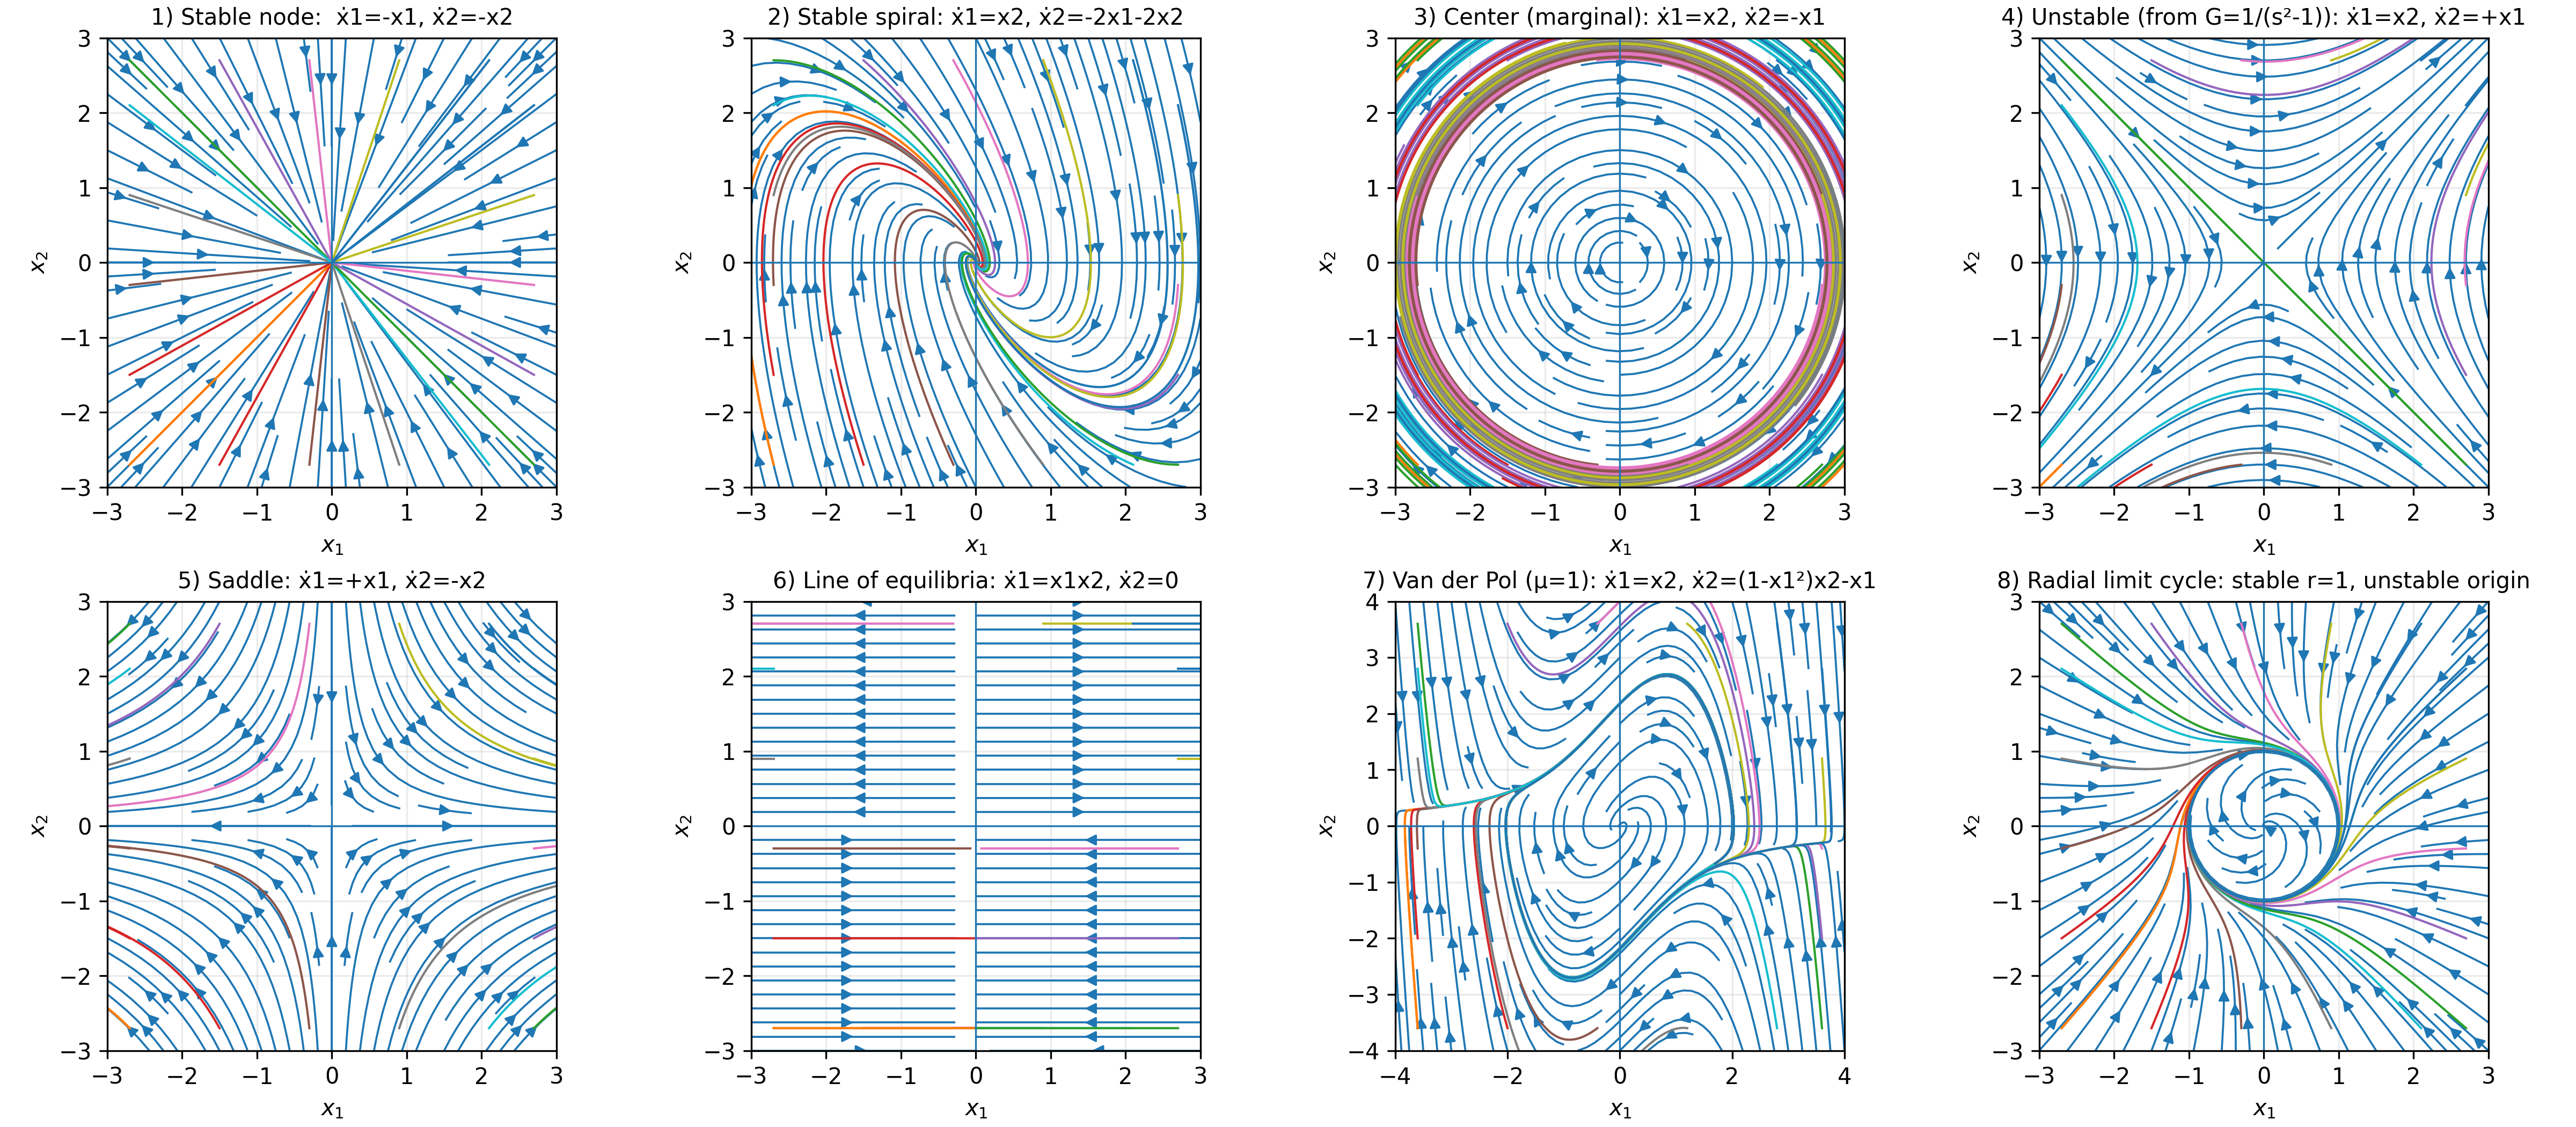
\includegraphics[width=\textwidth]{phase_portraits.png}
    \caption{Phase portraits for all eight systems in the worksheet (see below).}
    \label{fig:phase_portrait_example}
\end{figure}

Practice plotting phase portraits using the worksheet below using the steps for plotting phase portraits provided at the end of these notes.

\newpage 
% \pagestyle{empty}
\begin{landscape}

% ---------------- Page 1: 8 systems ----------------
\noindent
\textbf{Phase Portraits and Stability (Worksheet 2/25)}\hfill
Names (groups of 2):\ \rule{2in}{0.4pt}\hfill
Date:\ \rule{1.3in}{0.4pt}

\vspace{0.4em}
\noindent
For each system, your goal is to mark the equilibrium point(s) and sketch the phase portraits. Once you are done, add the title next to ``1'', ``2'' etc. to name the behavior of the system.

\vspace{0.6em}

\noindent
\portraitbox{1}{\dot x_1=-x_1\\ \dot x_2=-x_2}{}%
\portraitboxtf{2}{\dot x = \begin{bmatrix}0 & 1 \\ -2 & -2 \end{bmatrix}x + \begin{bmatrix}0 \\ 1 \end{bmatrix}u; y = x_2}{}%
\portraitbox{3}{\frac{Y(s)}{U(s)} = \frac{1}{s^2 + 1}}{}%
\portraitbox{4}{\dot x_1=x_2\\ \dot x_2=x_1}{}%

\vspace{0.8em}

\noindent
\portraitboxtf{5}{\dot x_1=x_1\\ \dot x_2=-x_2,\quad y = x_2}{}%
\portraitbox{6}{\dot x_1=x_1x_2\\ \dot x_2=0}{}%
\portraitbox{7}{\dot x_1=x_2\\ \dot x_2=(1-x_1^2)x_2-x_1}{}%
\portraitbox{8}{\dot x_1=x_2+x_1(1-x_1^2-x_2^2)\\ \dot x_2=-x_1+x_2(1-x_1^2-x_2^2)}{}%
\end{landscape}
\newpage

% ---------------- Page 2: instructions ----------------
\noindent\normalsize

\subsection*{Sketching Phase Portraits}\par

\textbf{Step 1:} Make sure to first rewrite the system model as:
\[
\dot x_1=f(x_1,x_2), \qquad \dot x_2=g(x_1,x_2).
\]

\textbf{Step 2:} Find the equilibrium point(s) of the system by solving
\[
f(x_1,x_2)=0,\qquad g(x_1,x_2)=0.
\]
Plot each equilibrium point on the phase plane with a ``$\times$'' mark.

% \textbf{Step 3: } If the system is nonlinear, linearize it by computing the Jacobian matrix:
% \[
% J(x_1,x_2)=
% \begin{bmatrix}
% \frac{\partial f}{\partial x_1} & \frac{\partial f}{\partial x_2}\\[4pt]
% \frac{\partial g}{\partial x_1} & \frac{\partial g}{\partial x_2}
% \end{bmatrix},
% \]
% and evaluate it at the equilibrium point(s) to get \(J^*\).

\textbf{Step 3:} Draw the nullclines, that is, the points at which the dynamics in each direction are zero:
\[
\text{\(x_1\)-nullcline: } f(x_1,x_2)=0 \quad (\dot x_1=0),
\qquad
\text{\(x_2\)-nullcline: } g(x_1,x_2)=0 \quad (\dot x_2=0).
\]


\textbf{Step 4:} Arrow directions of the nullclines can be computed by finding the sign of the dynamics (that is, the rate of change). Note that we write $\dot x = f(x, u)$ where the right hand side is the rate of change of the state. So, for positive values of the right hand side, the state is increasing, and for negative values, the state is decreasing. In particular, for each point in the phase plane, the direction of $x_1$ nullcline will be towards the right if $\dot x_1 > 0$ and towards the left if $\dot x_1 < 0$. Similarly, the direction of $x_2$ nullcline will be upwards if $\dot x_2 > 0$ and downwards if $\dot x_2 < 0$. 


\textbf{Step 5:} To predict the stability behavior, observe what the trajectories do as \(t\to\infty\):
\begin{itemize}
\item Asymptotically stable: trajectories near an equilibrium converge to it.
\item Marginally stable: trajectories remain nearby but do not converge. That is, if you are at the equilibrium, you will stay there, but if you are slightly away, you will not return to the equilibrium, but also not diverge away.
\item Unstable: some trajectories starting arbitrarily close move away in an unbounded fashion.
\item Limit cycle behavior: This is when orbits form! That is, the system exhibits periodic behavior, and trajectories converge to a closed curve in the phase plane. 
\end{itemize}

\end{document}